\documentclass{article}
\usepackage[top=1in, bottom=1in, left=1in, right=1in]{geometry}
\usepackage{polski}
\usepackage[utf8]{inputenc}
\usepackage{multirow}
\usepackage{graphicx}
\usepackage{float}
\begin{document}
\title{\huge\bfseries Wyznaczanie maksymalnej energii promieniowania
beta metodą absorpcyjną}
\date{}
\author{}
\maketitle
\section{Wstęp teoretyczny}
\subsection{Promieniowanie beta}
\textbf{Promieniowanie beta}\footnote[1]{https://pl.wikipedia.org/wiki/Promieniowanie\_beta, z dnia: 25.05.2017} to strumień elektronów lub pozytonów, emitowany przez jądra atomowe podczas przemiany jądrowej. Jest jednym z rodzajów promieniowania jonizującego oraz
jest bardziej przenikliwe od promieniowania alfa(przenikliwe czyli zdolne do przenikania przez różne materiały).
Energia promieniowania jest zależna od rodzaju źródła, a zasięg promieniowania dodatkowo od gęstości substancji absorbującej.\\\\
\textbf{Przykładowe źródła promieniowania beta:}
\begin{itemize}
\item promieniowanie sztucznych jądrach promieniotwórczych powstających podczas reakcji jądrowych
\item rozpad izotopu sodu 22Na
\end{itemize}
\subsection{Absorpcja promieniowania beta}
\textbf{Absorpcja promieniowania beta}\footnote[2]{https://pl.wikipedia.org/wiki/Absorpcja\_promieniowania\_beta, z dnia: 25.05.2017} jest to proces pochłaniania promieniowania przez substancję. Oddziaływanie promieniowania beta z materią powoduje straty energii cząstek beta oraz zmianę toru ich ruchu.\\\\
\textbf{Zasięg masowy promieniowania}\footnote[3]{https://pl.wikipedia.org/wiki/Oslona\_przed\_promieniowaniem, z dnia: 25.05.2017} jest zależny od energii cząsteczek beta, czyli od zasięgu maksymalnego dla danego izotopu pierwiastka promieniotwórczego oraz od współczynnika pochłaniania absorbującej materii.
\section{Przebieg i cel ćwiczenia}
Celem ćwiczenia jest wyznaczenie maksymalnej energii promieniowania beta metodą absorpcyjną.
\subsection{Tabele pomiarowe}
\newpage
\begin{table}
\centering
\label{my-label}
\begin{tabular}{|c|c|}
\hline
$N_T$                                                            & $99$  \\ \hline
$t, min$                                                        & $10$  \\ \hline
\begin{tabular}[c]{@{}l@{}}Poziom tła\\ $I_T=N_T/t$ imp$/$min,\end{tabular} & $9,9$ \\ \hline
\end{tabular}
\end{table}

\begin{table}[]
\centering
\label{my-label}
\begin{tabular}{|c|c|c|c|}
\hline
\begin{tabular}[c]{@{}c@{}}grubość\\ $x, mm$\end{tabular} & \begin{tabular}[c]{@{}c@{}}ilość\\ impulsów N\end{tabular} & \begin{tabular}[c]{@{}c@{}}czas\\ $t, min$\end{tabular} & \begin{tabular}[c]{@{}c@{}}$I=N/t$\\ $imp/min$\end{tabular} \\ \hline
0                                                       & 1000                                                       & 0,69                                                  & 1449,28                                                 \\ \hline
0,05                                                    & 1000                                                       & 1,16                                                  & 862,07                                                  \\ \hline
0,10                                                    & 1000                                                       & 1,56                                                  & 641,03                                                  \\ \hline
0,15                                                    & 1000                                                       & 2,06                                                  & 485,44                                                  \\ \hline
0,20                                                    & 1000                                                       & 2,96                                                  & 337,84                                                  \\ \hline
0,25                                                    & 1000                                                       & 3,69                                                  & 271,00                                                  \\ \hline
0,30                                                    & 1000                                                       & 4,77                                                  & 209,64                                                  \\ \hline
0,35                                                    & 1000                                                       & 6,28                                                  & 159,24                                                  \\ \hline
0,40                                                    & 1000                                                       & 8,19                                                  & 122,19                                                  \\ \hline
0,45                                                    & 1000                                                       & 10,97                                                 & 91,16                                                   \\ \hline
0,50                                                    & 1000                                                       & 14,33                                                 & 69,78                                                   \\ \hline
\end{tabular}
\end{table}
\subsection{Opracowanie wyników pomiarów}
Obliczyliśmy niepewność $u(I)$ korzystając z prawa propagacji niepewności
$$u(I) = \sqrt{(\frac{1}{T} \cdot u(N)^2 + (-\frac{N}{T^2} \cdot u(T))^2}$$
gdzie $u(N) = \sqrt{1000} \approx 31,62$ , a $u(T) = \frac{1}{60}$ czyli jest to 1 sekunda.\\
Np. dla $N = 1000$ oraz $T = 4,77$
$$u(I) = \sqrt{(\frac{1}{4,77} \cdot 31,62)^2 + (-\frac{1000}{4,77^2} \cdot \frac{1}{60})^2} = 6,669$$ 
Niepewność grubości absorbenta to $10\mu m$ wynikająca z niepewności sprzętu, którym był on mierzony.
Sporządziliśmy wykres zależności natężenia wiązki do grubości absorbenta $I = f(x)$
\begin{figure}[ht]
\caption{Zależność natężenia wiązki od grubości absorbenta}
\centering
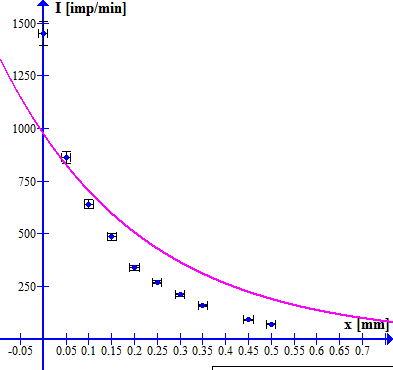
\includegraphics{wykres_1.png}
\end{figure}
Przekształciliśmy wzór 
$$I = I_0e{-x\mu }$$ 
do postaci
$$lnI = - x\mu + lnI_0 $$
Ukazuje on nam zależność liniową pomiędzy $lnI$, a grubością absorbenta $x$
Współczynniki zależności wyliczyliśmy korzystając z funkcji REGLINP(MS Excel), i tak:
$$a = -3,27(28)$$
$$b = 6,88(11)$$
Obliczyliśmy logarytm naturalny z wartości $I$
$$u(lnI) = \frac{1}{I} \cdot u(I)$$
\begin{center}
    \begin{tabular}{|c|c|}
        \hline 
        $I [imp/min]$ & $ln(I)$ \\ \hline
        $1449,28$ & $7,278(39)$ \\ \hline
        $862,07$ & $6,759(35)$ \\ \hline
        $641,03$ & $6,463(34)$ \\ \hline
        $485,44$ & $6,185(34)$ \\ \hline
        $337,84$ & $5,822(33)$ \\ \hline
        $271$ & $5,602(32)$ \\ \hline
        $209,64$ & $5,345(31)$ \\ \hline
        $159,24$ & $5,070(31)$ \\ \hline
        $12219$ & $9,4101(31)$ \\ \hline
        $91,16$ & $4,512(31)$ \\ \hline
        $69,78$ & $4,245(31)$ \\ \hline  
    \end{tabular}
\end{center}
Sporządziliśmy wykres zależności logarytmu naturalnego z ilością zliczeń w jednostce czasu od grubości absorbenta
\begin{figure}[ht]
\caption{Zależności logarytmu naturalnego z ilością zliczeń w jednostce czasu od grubości absorbenta}
\centering
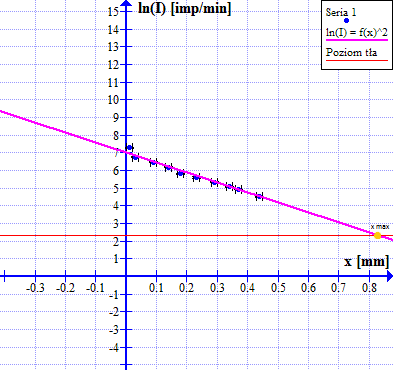
\includegraphics{wykres_2.png}
\end{figure}
Na wykresie została również ukazana prosta $ln(I_T)$ czyli logarytm naturalny ilości zliczeń poziomu tła.
Współczynnik 
$$\mu = -a = 3,27(28)\ [1/mm]$$
Punkt przecięcia prostej $y = ln(I_T)$ oraz prostej wyznaczonej powyższej zależności wyznacza nam zasięg maksymalny promieniowania 
$$x_{max} = \frac{ln(I_0) - ln(I_T)}{\mu} = \frac{ln(I_T) - b}{a} = 0,84\ [mm]$$
Metodą propagacji niepewności obliczamy 
$$u(x_{max}) = \sqrt{(\frac{1}{I_Ta} \cdot u(I_T))^2 + (-\frac{1}{a} \cdot u(b))^2 + (\frac{a - ln(I_T)}{a^2} \cdot u(a))^2}$$
więc,
$$x_{max} = 0,84(7)\ [mm]$$
\end{document}